\documentclass[12pt,a4paper]{article}

\usepackage{fontspec}
\usepackage{polyglossia}
\setmainlanguage{russian}
\setotherlanguage{english}
\setmainfont{DejaVu Serif}
\setsansfont{DejaVu Sans}
\setmonofont{DejaVu Sans Mono}

\usepackage{amsmath}
\usepackage{amssymb}
\usepackage{graphicx}
\usepackage{geometry}
\usepackage{booktabs}
\usepackage{listings}
\usepackage{xcolor}
\usepackage{hyperref}

\geometry{a4paper, margin=2.5cm}
\hypersetup{colorlinks=true, linkcolor=blue, urlcolor=blue}

\definecolor{codebg}{RGB}{245,245,245}
\lstset{
    backgroundcolor=\color{codebg}, basicstyle=\ttfamily\small,
    breaklines=true, frame=single, showstringspaces=false,
    keywordstyle=\color{blue}, commentstyle=\color{gray},
}

\title{Отчёт по лабораторной работе №2 \\ \large Продвинутые методы оптимизации}
\author{}
\date{}

\begin{document}
\maketitle
\tableofcontents
\newpage

\section{Постановка задачи}

Цель работы -- реализовать два стохастических метода оптимизации, не
требующих непрерывности целевой функции, поверх типа
\texttt{ConstructiveNumber} из лабораторной работы №1, протестировать
их на функциях с разной степенью сложности (гладкая мультимодальная,
гладкая с плоской периферией, разрывная) и сравнить со скоростью
сходимости, числом вызовов функции и требуемой памятью методов лабы 1.

\section{Интервальные elementary-функции}

Тестовые функции этой лабы используют $\cos$, $\sin$, $\exp$, $\sqrt{\ }$,
$\mathrm{round}$ -- в лабе 1 такие функции не требовались (там были только
$+,-,\times,/$), поэтому пришлось реализовать их интервальные версии.

\textbf{Монотонные функции} ($\exp$, $\sqrt{\ }$): интервальное расширение
тривиально -- $f([a,b])=[f(a),f(b)]$, поскольку монотонность гарантирует,
что экстремумы достигаются на границах.

\textbf{$\cos$ и $\sin$ не монотонны} -- нужно проверить, не попадает ли
внутрь отрезка $[a,b]$ точка экстремума (для $\cos$ -- максимум в точках
$2\pi k$, минимум в $\pi+2\pi k$). Если попадает -- результат обязан
включать этот экстремум ($1$ или $-1$), иначе интервал будет неверно
узким. Если нет -- достаточно $\min$/$\max$ от значений на границах.
$\sin$ реализован через сдвиг фазы: $\sin(x)=\cos(x-\pi/2)$.

\textbf{$\mathrm{round}$ разрывна} -- интервальное расширение обязано
быть \emph{консервативным}: возвращает весь диапазон целых чисел,
которые может дать округление любой точки внутри $[a,b]$.

\section{Тестовые функции}

\begin{table}[h]
\centering
\begin{tabular}{lll}
\toprule
Функция & Гладкость & Основная сложность \\
\midrule
Rastrigin-2 & гладкая & $\approx$400 локальных минимумов на $[-5.12,5.12]^2$ \\
Ackley-2 & гладкая & почти нулевой градиент на периферии \\
Desmos & \textbf{не гладкая} & разрывы из-за $\mathrm{round}(\cdot)$, градиент не определён \\
\bottomrule
\end{tabular}
\caption{Тестовые целевые функции лабы 2}
\end{table}

\begin{align}
f_{\mathrm{Rastrigin}}(x,y) &= 20 + x^2-10\cos(2\pi x) + y^2-10\cos(2\pi y) \\
f_{\mathrm{Ackley}}(x,y) &= -20\exp\!\left(-0.2\sqrt{\tfrac{x^2+y^2}{2}}\right)
    -\exp\!\left(\tfrac{\cos2\pi x+\cos2\pi y}{2}\right)+e+20 \\
f_{\mathrm{Desmos}}(x,y) &= \big(x(\mathrm{round}(\sin10y)+2)+y-10\big)^2
    + \big(x+(y(\mathrm{round}(\sin7x)+2))^2-7\big)^2
\end{align}

Глобальный минимум всех трёх функций -- $f=0$ в точке $(0,0)$ (для
Desmos -- приближённо).

\section{Методы оптимизации}

\subsection{Имитация отжига (Simulated Annealing)}

На каждом шаге пробуется случайный "сосед" $y$ в радиусе $\delta$ от
текущей точки $x^*$. Если $y$ лучше -- переход происходит всегда. Если
хуже -- переход происходит с вероятностью Метрополиса:
\begin{equation}
    p(x,y,t) = \exp\!\left(\frac{f(x)-f(y)}{t}\right)
\end{equation}
Температура $t$ постепенно остывает: $t \leftarrow t\cdot\gamma$,
$\gamma<1$, на каждой итерации. Готовность иногда "ухудшиться" позволяет
методу выбраться из локальных минимумов -- пока температура высокая,
такие переходы происходят часто; к концу работы метод становится
разборчивее.

\subsection{Генетический алгоритм}

Поддерживается популяция из $k$ точек. На каждом поколении:
\begin{enumerate}
    \item \textbf{Отбор (selection)} -- турнирный: берём случайных
    \texttt{tournament\_size} особей, оставляем лучшую; повторяем $r$ раз.
    \item \textbf{Скрещивание (crossover)} -- новая особь = среднее
    арифметическое двух случайно выбранных родителей.
    \item \textbf{Мутация} -- с вероятностью \texttt{mutation\_rate} к
    каждой координате потомка добавляется гауссов шум.
\end{enumerate}

\section{Результаты исследования}

\subsection{Сравнение на функциях лабы 1 (гладкие)}

\begin{table}[h]
\centering
\small
\begin{tabular}{llccccc}
\toprule
Функция & Метод & Итер. & func\_calls & Время,с & Память & $f_{min}$ \\
\midrule
QuadraticGood & Град.спуск & 1625 & 1625 & 0.032 & 587 KB & $5.0\times10^{-13}$ \\
QuadraticGood & Нелдера-Мида & 230 & 374 & 0.013 & 56 KB & $4.8\times10^{-9}$ \\
QuadraticGood & Имит.отжига & 3000 & 3001 & 0.037 & 891 KB & $6.9\times10^{-2}$ \\
QuadraticGood & Генетич.алг. & 150 & 6040 & 0.166 & 34 KB & $3.2\times10^{-4}$ \\
QuadraticBad & Град.спуск & 1536 & 1536 & 0.024 & 428 KB & $5.0\times10^{-13}$ \\
QuadraticBad & Нелдера-Мида & 158 & 269 & 0.007 & 29 KB & $1.3\times10^{-8}$ \\
QuadraticBad & Имит.отжига & 3000 & 3001 & 0.030 & 686 KB & $1.1\times10^{-1}$ \\
QuadraticBad & Генетич.алг. & 150 & 6040 & 0.135 & 27 KB & $1.8\times10^{-4}$ \\
Rosenbrock & Град.спуск & 20000 & 20000 & -- & -- & $4.8\times10^{-9}$ \\
Rosenbrock & Нелдера-Мида & 223 & 392 & 0.007 & 35 KB & $3.3\times10^{-9}$ \\
Rosenbrock & Имит.отжига & 3000 & 3001 & 0.024 & 471 KB & $4.96\times10^{-1}$ \\
Rosenbrock & Генетич.алг. & 150 & 6040 & 0.128 & 25 KB & $7.2\times10^{-1}$ \\
\bottomrule
\end{tabular}
\caption{Сравнение всех 4 методов на функциях лабы 1}
\end{table}

\textbf{Вывод:} на гладких функциях детерминированные методы (особенно
градиентный спуск) существенно точнее ($\sim10^{-13}$ против
$\sim10^{-1}$ у стохастических) при сопоставимом или меньшем числе
вызовов функции -- ожидаемо, поскольку градиентный спуск использует
дополнительную информацию (производную).

\begin{figure}[h]
    \centering
    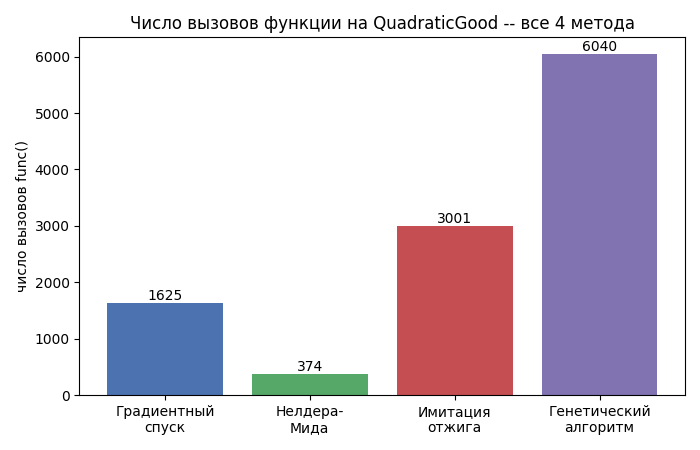
\includegraphics[width=0.7\textwidth]{../img/func_calls_comparison.png}
    \caption{Число вызовов функции по всем 4 методам на QuadraticGood.}
\end{figure}

\clearpage
\subsection{Сравнение на функциях лабы 2}

Градиентный спуск здесь неприменим в принципе -- при попытке вызова
метод возвращает \texttt{NotImplementedError} (аналитический градиент
для этих функций сознательно не реализован).

\begin{table}[h]
\centering
\begin{tabular}{llccc}
\toprule
Функция & Метод & Итераций & func\_calls & $f_{min}$ \\
\midrule
Rastrigin-2 & Нелдера-Мида & 45 & $\sim$90 & 4.97 \\
Rastrigin-2 & Имитация отжига & 5000 & 5001 & 0.022 \\
Rastrigin-2 & Генетический алг. & 200 & 8040 & 0.00003 \\
Ackley-2 & Имитация отжига & 5000 & 5001 & 0.023 \\
Ackley-2 & Генетический алг. & 200 & 8040 & 0.00035 \\
Desmos & Нелдера-Мида & 133 & $\sim$260 & 0.042 \\
Desmos & Имитация отжига & 5000 & 5001 & 26.6 \\
Desmos & Генетический алг. & 200 & 8040 & 0.00027 \\
\bottomrule
\end{tabular}
\caption{Сравнение методов на функциях лабы 2}
\end{table}

\textbf{Ключевое наблюдение:} метод Нелдера-Мида мгновенно застревает на
Растригине (45 итераций, далеко от глобального минимума) -- классическая
ловушка локального метода на мультимодальной функции с $\sim$400 ямами.
Генетический алгоритм стабильно находит глобальный минимум на всех трёх
функциях, включая недифференцируемую Desmos.

\subsection{Устойчивость имитации отжига к случайности}

Запустили имитацию отжига на Rastrigin-2 десять раз с разными \texttt{seed}.

\begin{figure}[h]
    \centering
    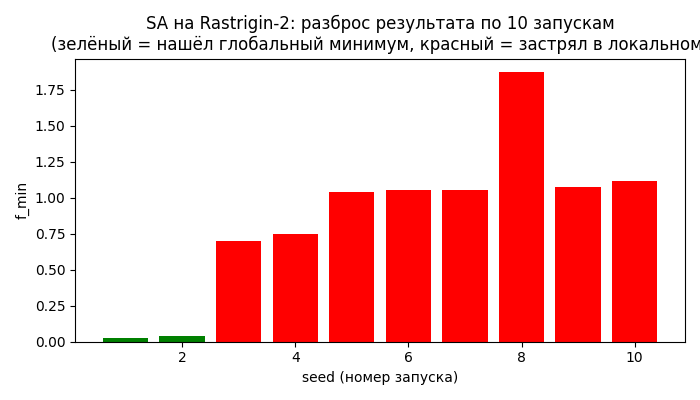
\includegraphics[width=0.7\textwidth]{../img/sa_seed_variance.png}
    \caption{Только 2 из 10 запусков (20\%) нашли глобальный минимум --
    остальные застряли в одном из соседних локальных минимумов.}
\end{figure}

\begin{figure}[h]
    \centering
    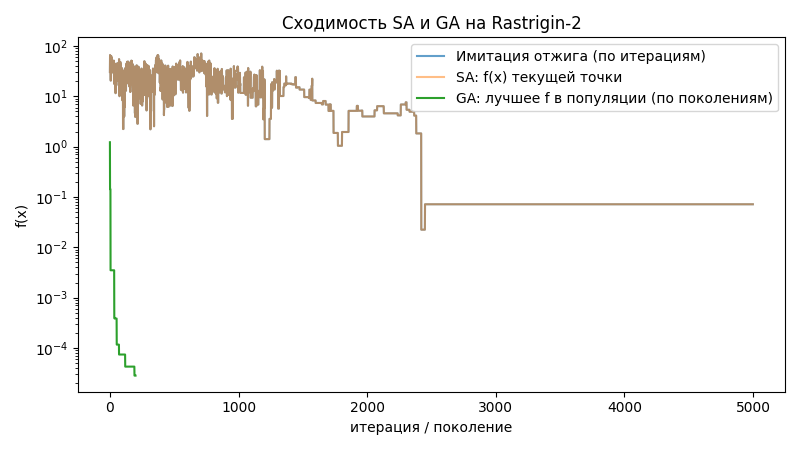
\includegraphics[width=0.75\textwidth]{../img/convergence_sa_ga_rastrigin.png}
    \caption{Сходимость SA (шумная траектория, постоянные колебания) и
    GA (плавная, быстрая сходимость за $\sim$150--200 поколений).}
\end{figure}

\clearpage
\section{Теоретическое объяснение}

Имитация отжига исследует пространство \textbf{одной точкой} -- если эта
точка попадает в область притяжения локального минимума после того, как
температура уже остыла, шанс выбраться оттуда стремится к нулю.
Генетический алгоритм одновременно поддерживает \textbf{целую популяцию}
точек -- даже если большинство особей застревает в разных локальных
минимумах, скрещивание между разными "удачными" особями может дать
потомка ближе к глобальному минимуму. Это структурное преимущество
популяционного поиска особенно заметно на функциях с большим числом
локальных минимумов (Растригин) -- SA имеет только один шанс не
застрять, GA -- сразу несколько параллельных попыток.

С другой стороны, GA требует существенно больше вызовов функции на
итерацию (весь размер популяции на каждое поколение), что видно и в
таблицах, и на графике сравнения -- это плата за более широкое
исследование пространства.

\section{Заключение}

Детерминированные методы лабы 1 эффективнее там, где применимы (гладкие
функции с известным градиентом или простой унимодальной структурой) --
дают существенно более точный результат при сопоставимых затратах.
Стохастические методы лабы 2 необходимы там, где детерминированные
неприменимы или ненадёжны: недифференцируемые функции и функции с
большим числом локальных минимумов. Среди двух стохастических методов
генетический алгоритм оказался надёжнее имитации отжига на всех трёх
тестовых функциях этой лабы -- ценой большего числа вызовов функции на
итерацию.

\end{document}
